	\section{Extrsuor}
	\subsection{Material necesario}
		\begin{itemize}
			\item Piezas impresas Extrusor
			\item 3x rodamientos axiales
			\item 1x tuerca M8.
			\item 2x tuercas autoblocantes M8.
			\item 4x arandelas M8.
			\item 2x muelles 25mm.
			\item 3x tonillos M3x30.
			\item 2x tornillos M3x15
			\item 3x tornillos M3x10.
			\item 2x varillas roscadas M4.
			\item 2x palometas M4.
			\item 2x tuercas M4.
			\item 1x varilla lisa M8x10.
		\end{itemize}
		\begin{figure}[!htp]
			\centering
			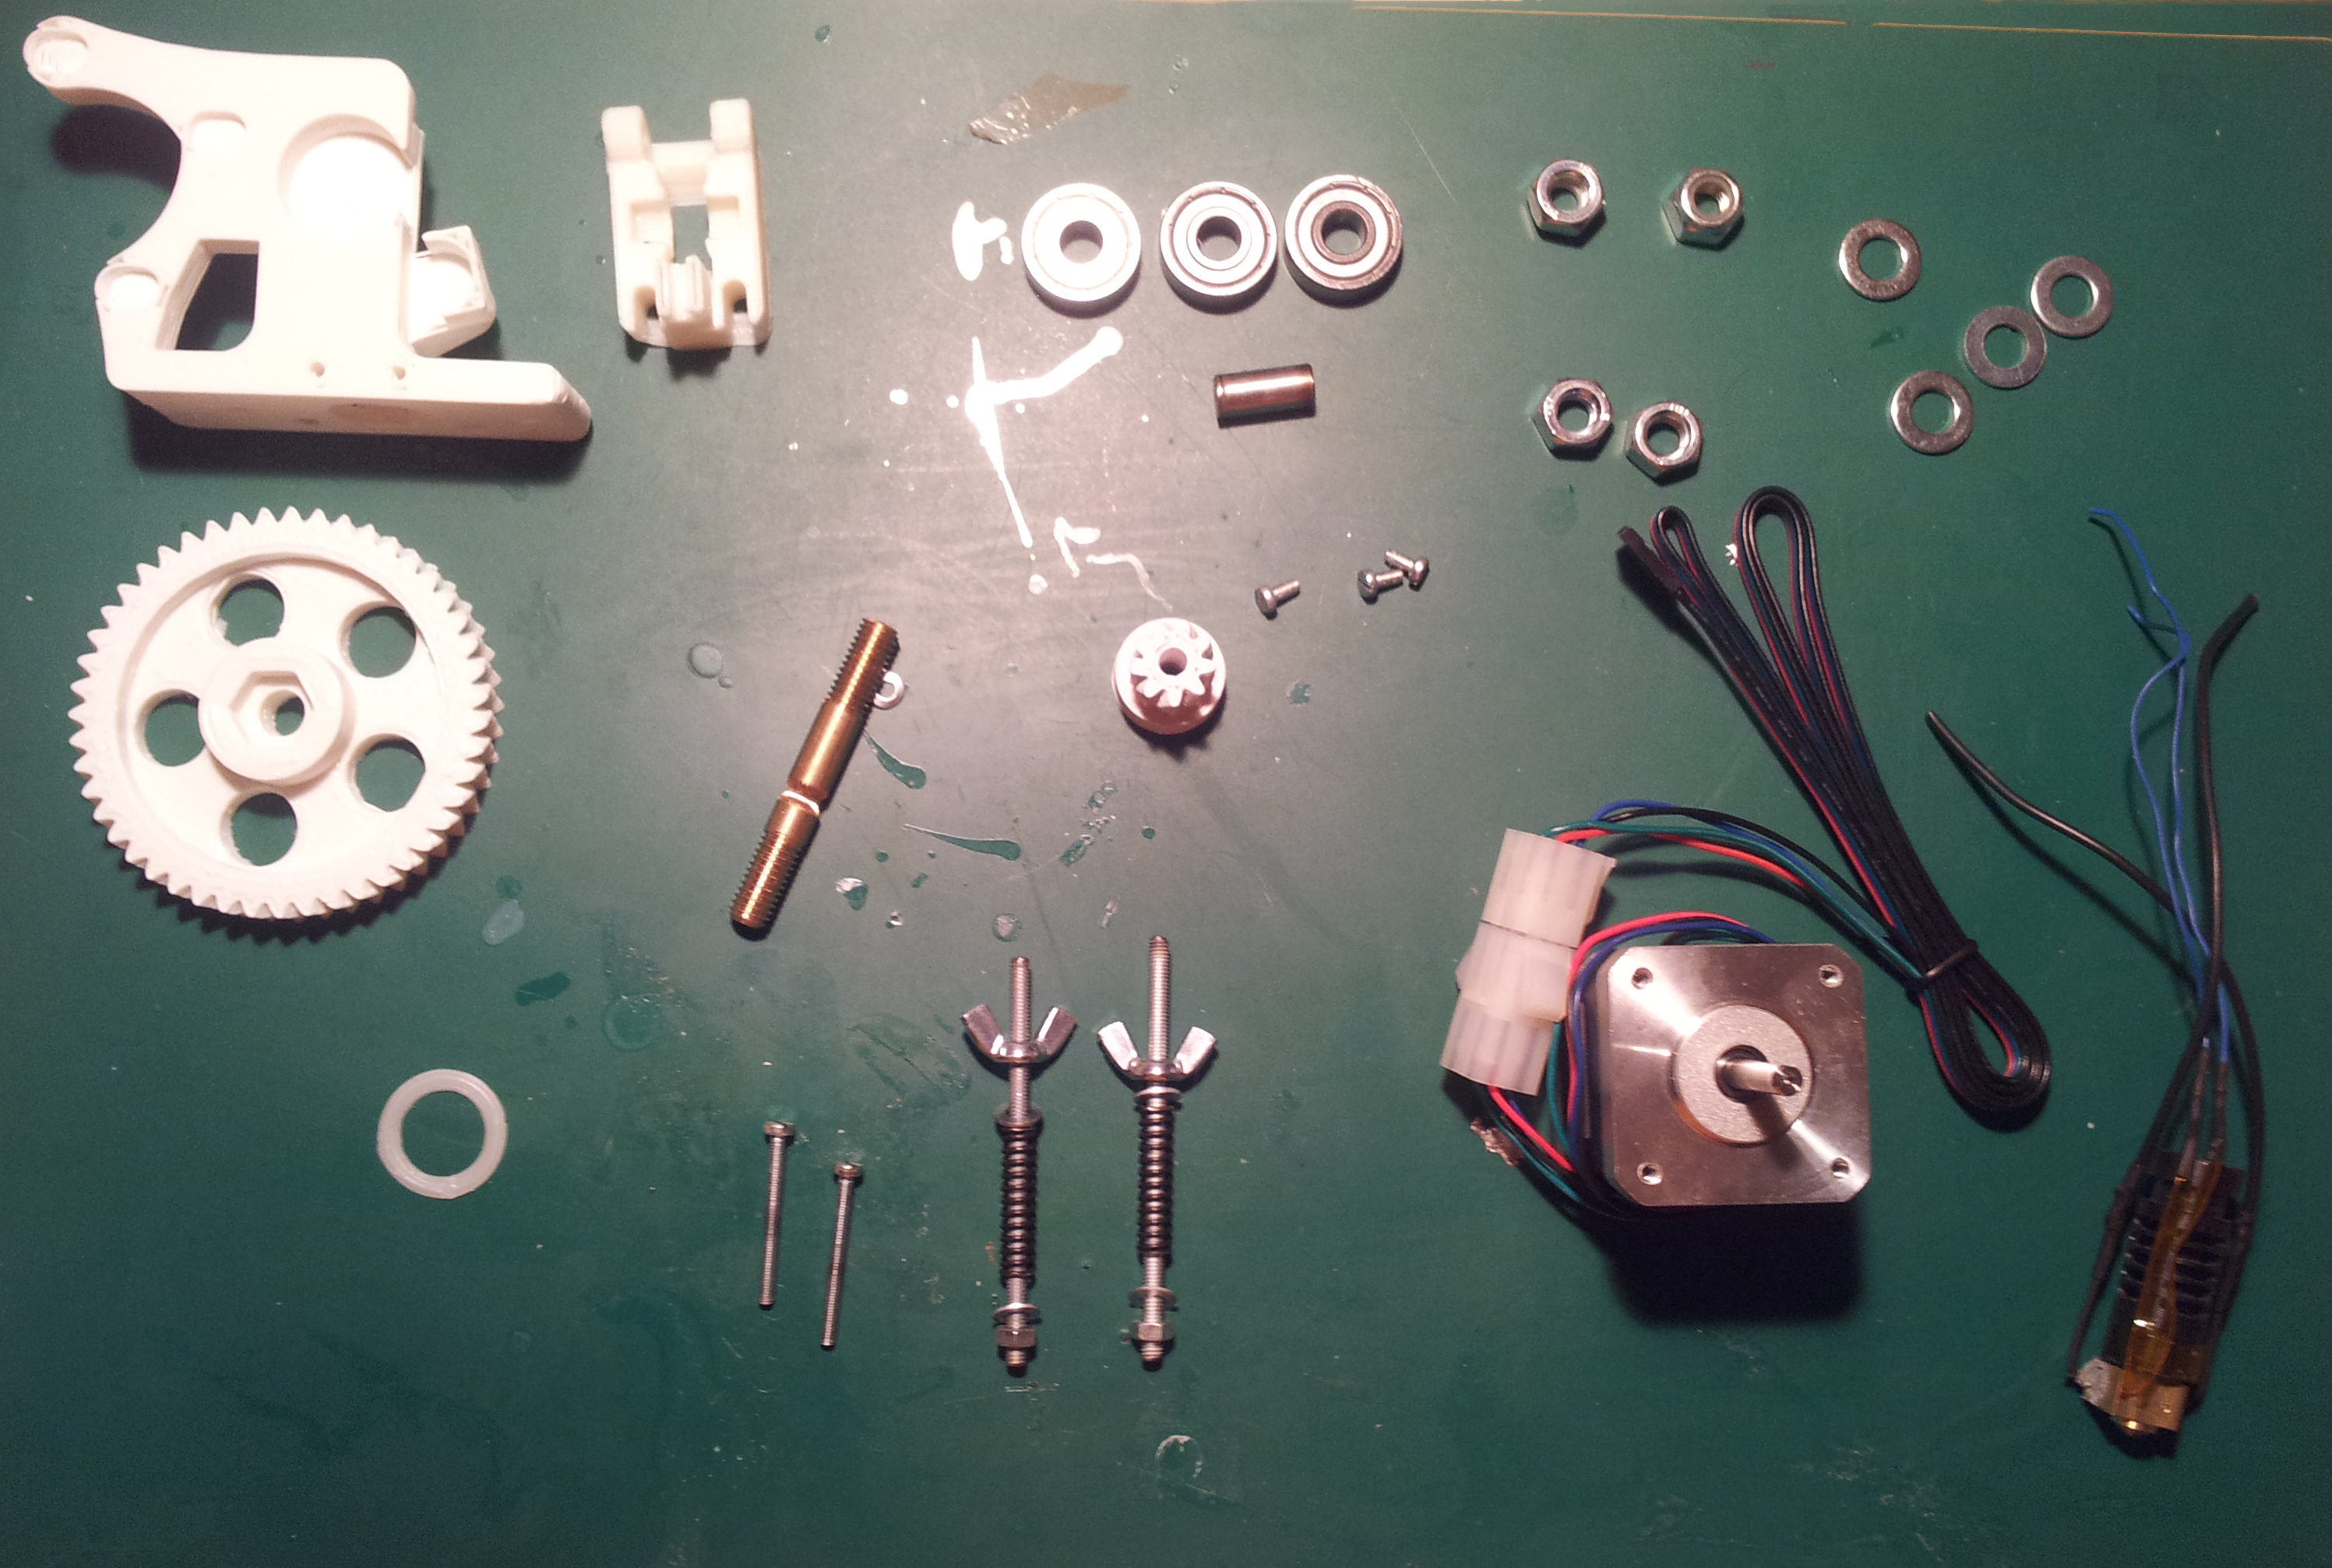
\includegraphics[width=0.7\textwidth]{../../Fotos/95.jpg}
			\caption{Material necesario}
		\end{figure}
		\newpage{}
	\subsection{Herramienta necesaria}
		\begin{itemize}
			\item Alicates de punta fina.
			\item Alicates de corte o tijeras.
			\item Destornillador.
			\item Llave inglesa para M8.
			\item Destornilladores.
			\item Lima fina.
		\end{itemize}
		\begin{figure}[!htp]
			\centering
			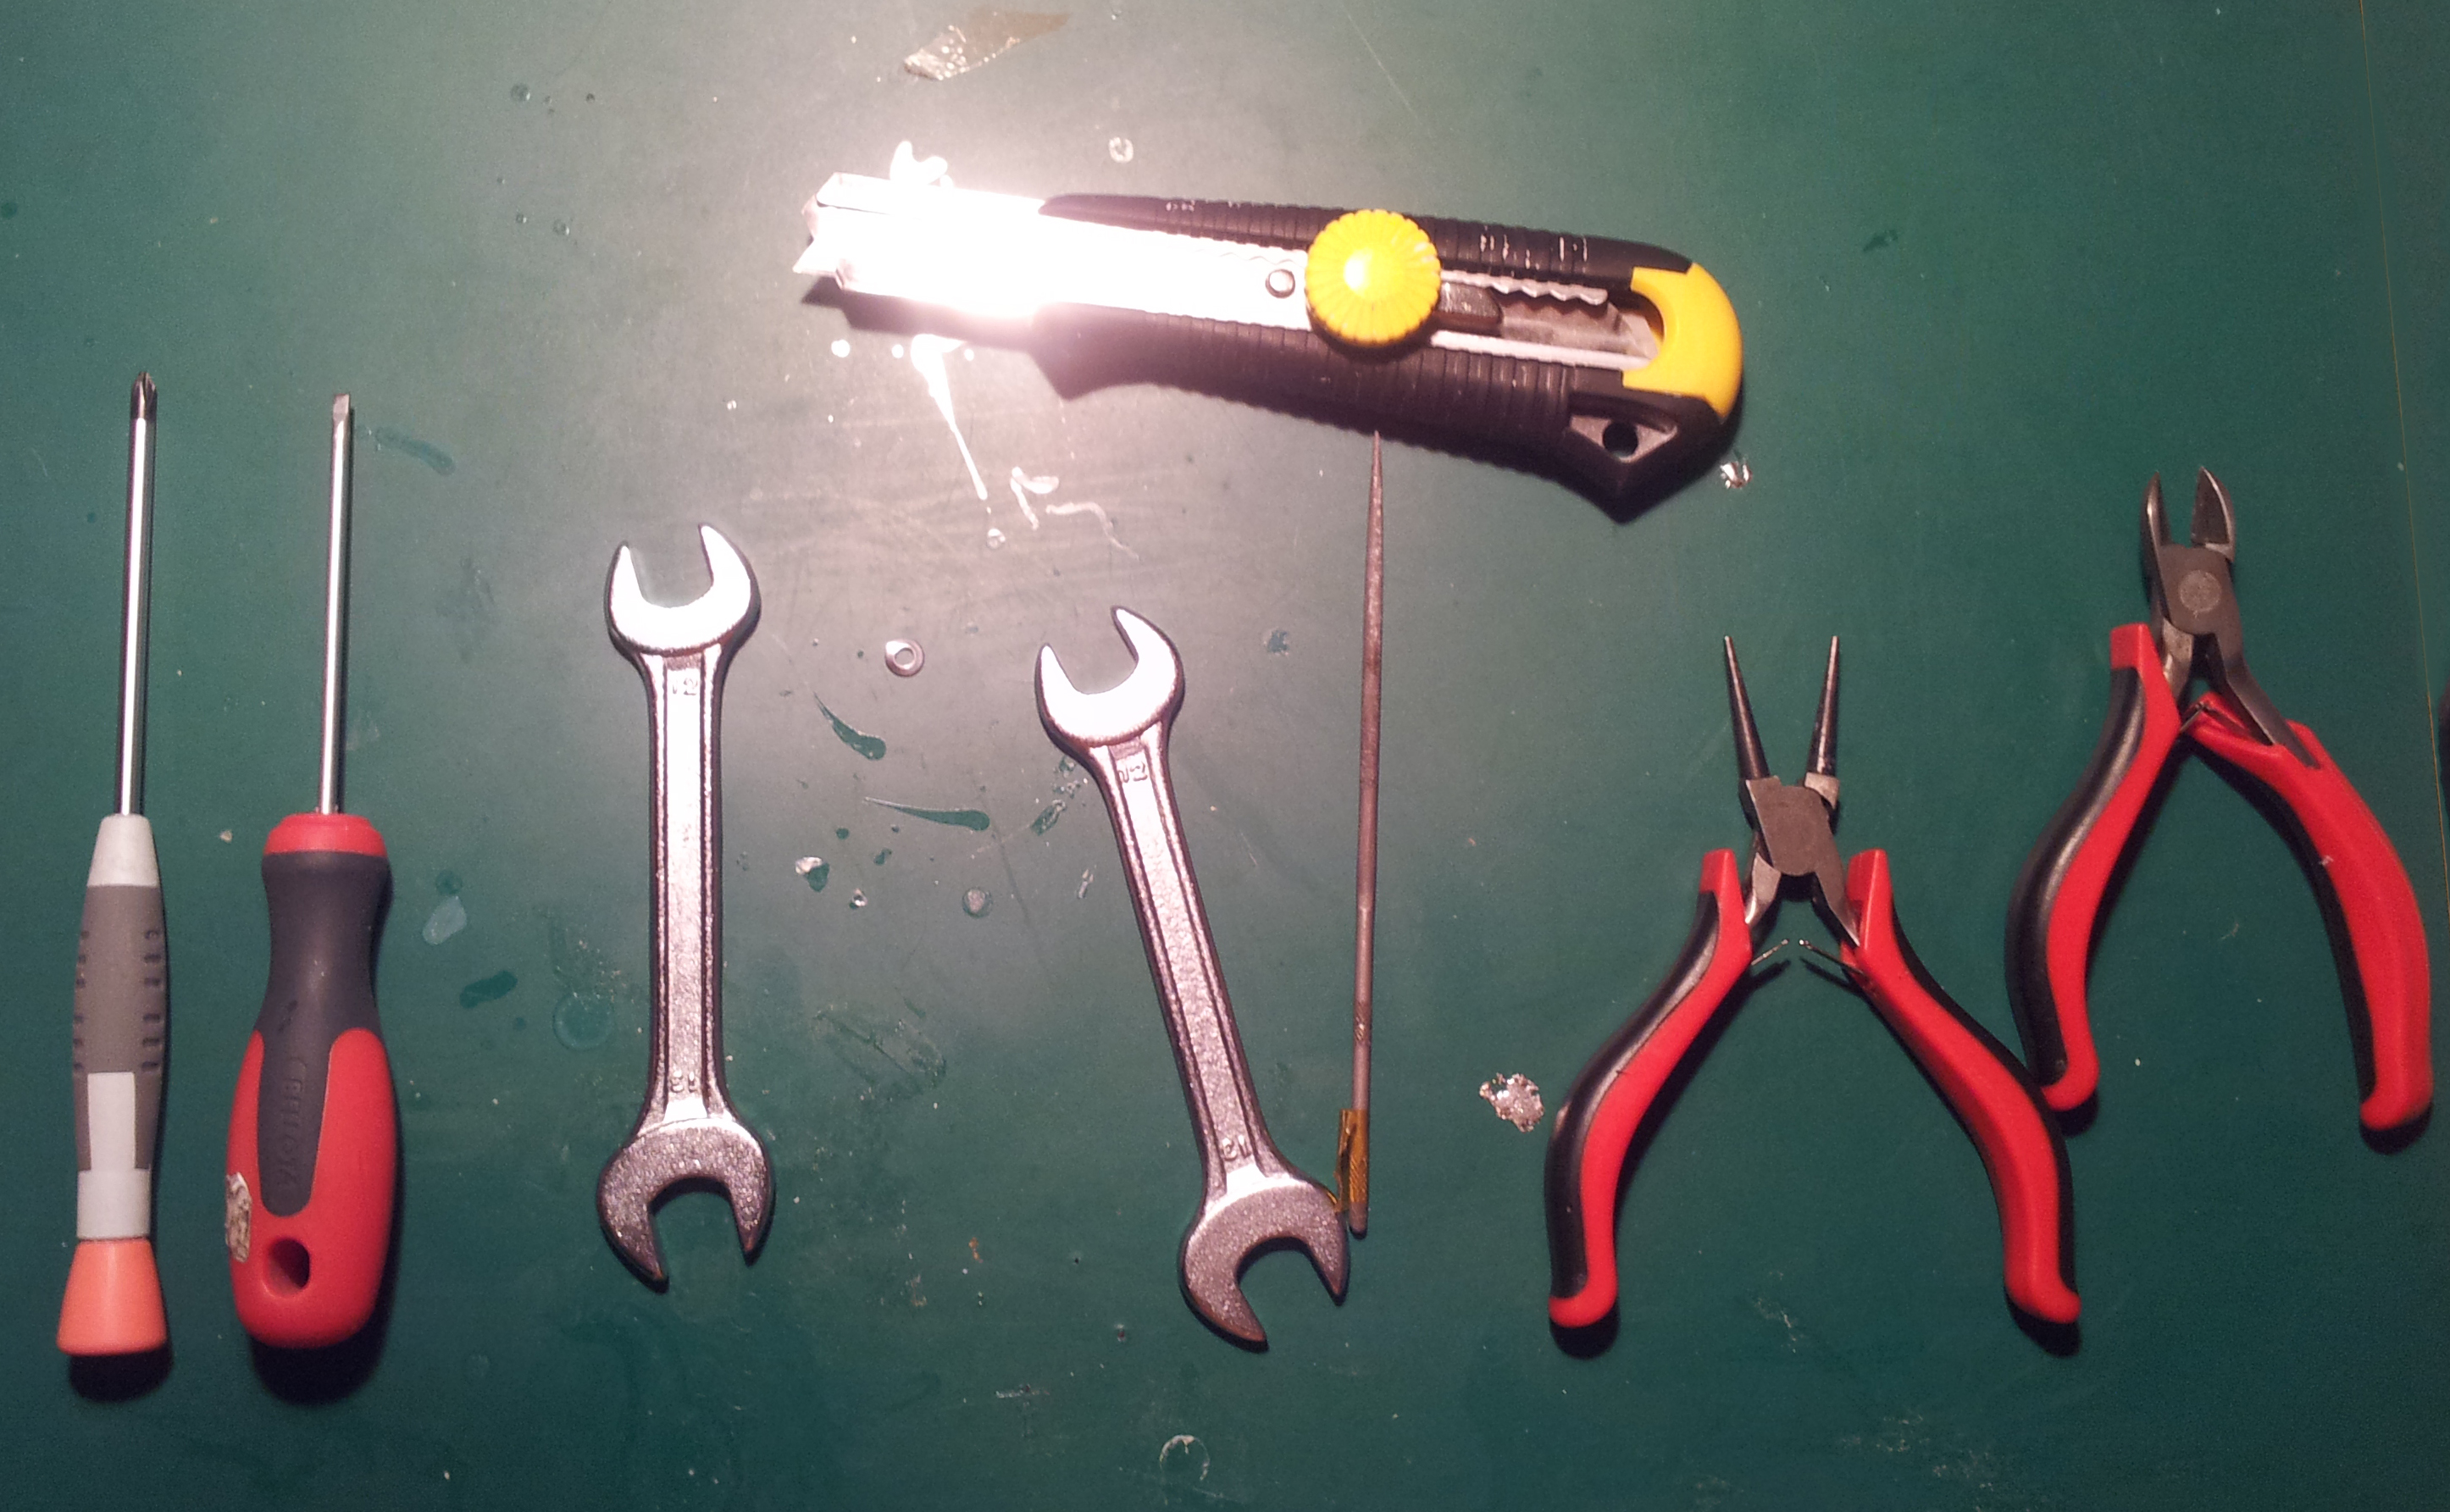
\includegraphics[width=0.7\textwidth]{../../Fotos/96.jpg}
			\caption{Herramienta necesaria}
		\end{figure}
		
		\newpage{}
			\subsection{Operativa}
			Primero vamos a preparar el hotend. Introducimos la resistencia en el agujero, haciendo que sobresalga una patilla por cada lado, y pegandola con masilla. A continuacion, forramos las patillas del termistor con capton (dejando la punta libre) y lo
			introducimos en el ajugero correspondiente, sujetandolo con capton alrededor del hotend.\\
			Soldamos un cable de de 2 puntas a los exremos del termistor, y el cable grueso a las de la resistencia.\\
			
			\begin{figure}[!htp]
				\centering
				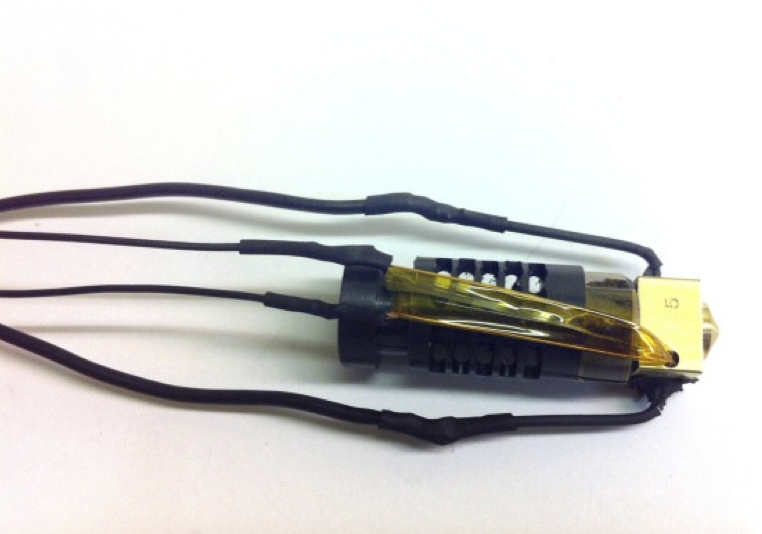
\includegraphics[width=0.7\textwidth]{../../Fotos/97.jpg}
				\caption{Hotend}
			\end{figure}
			
				Vamos a preparar ahora las piezas de plastico. Insertamos una tuerca M8 autoblocante en el agujero del engranaje grande. A continuacion colocamos dos rodamientos en los ajugeros del cuerpo del extrusor. Enroscamos el tornillo extrusor Hyena en el	engranaje, hasta que sobresalga un poco. Colocamos dos arandelas en el tornillo extrusor y lo introducimos por los dos rodamientos tal y como aparece en la imagen ~\ref{fig:1.ext}
			\begin{figure}[!htp]
				\centering
				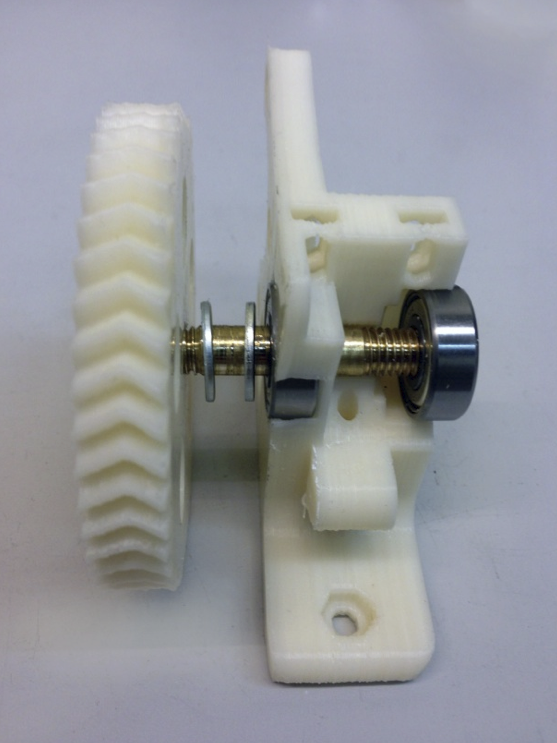
\includegraphics[width=0.7\textwidth]{../../Fotos/98.jpg}
				\caption{Extrusor con tornillo}
				\label{fig:1.ext}
			\end{figure}
			\begin{figure}[!htp]
				\centering
			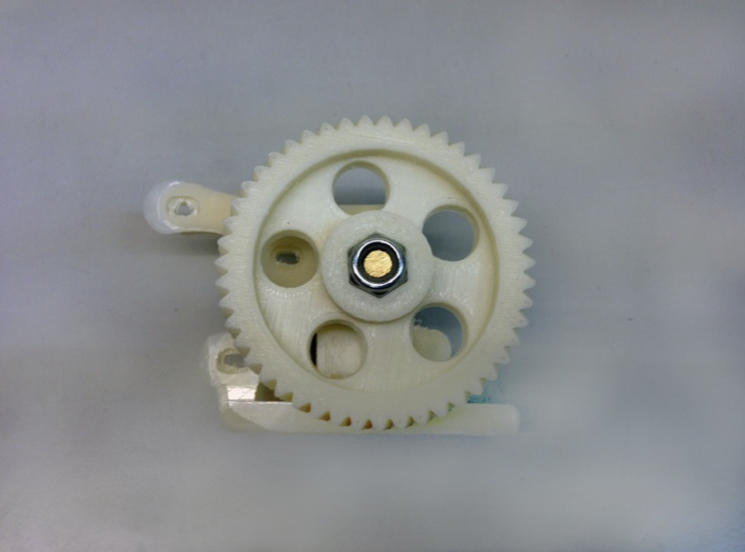
\includegraphics[width=0.7\textwidth]{../../Fotos/99.jpg}
			\caption{Frontal Extrusor}
			\label{fig:2.ext}
		\end{figure}
		La muesca del tornillo extrusor debe coincidir justo encima del ajugero por el que pasa el filamento. Si no es asi, enroscar más el tornillo extrusor, o añadir una arandela más.\\
		A continuación arrancamos el pequeño soporte de plástico del cuerpo del extrusor, e introducimos el pequeño trozo de varilla roscada, con un rodamiento, en el extruder idler. Colocamos el extruder idler, sujetándolo con un tornillo M3x40 al cuerpo del extrusor. Colocamos también las varillas roscadas pequeñas con la palometa y el muelle tal y como aparece en la imagen.\\
		Después introducimos otra tuerca autoblocante M8 por la otra parte del tornillo extrusor Hyena, sin apretarla demasiado para que el engranaje gire libremente, pero sin desplazarse\\
		\begin{figure}[!htp]
			\centering
		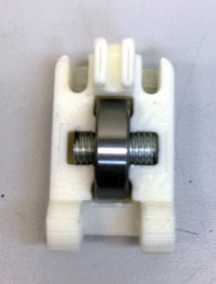
\includegraphics[width=0.7\textwidth]{../../Fotos/100.jpg}
		\caption{ Idler Extrusor}
		\label{fig:3.ext}
	\end{figure}
	\begin{figure}[!htp]
		\centering
	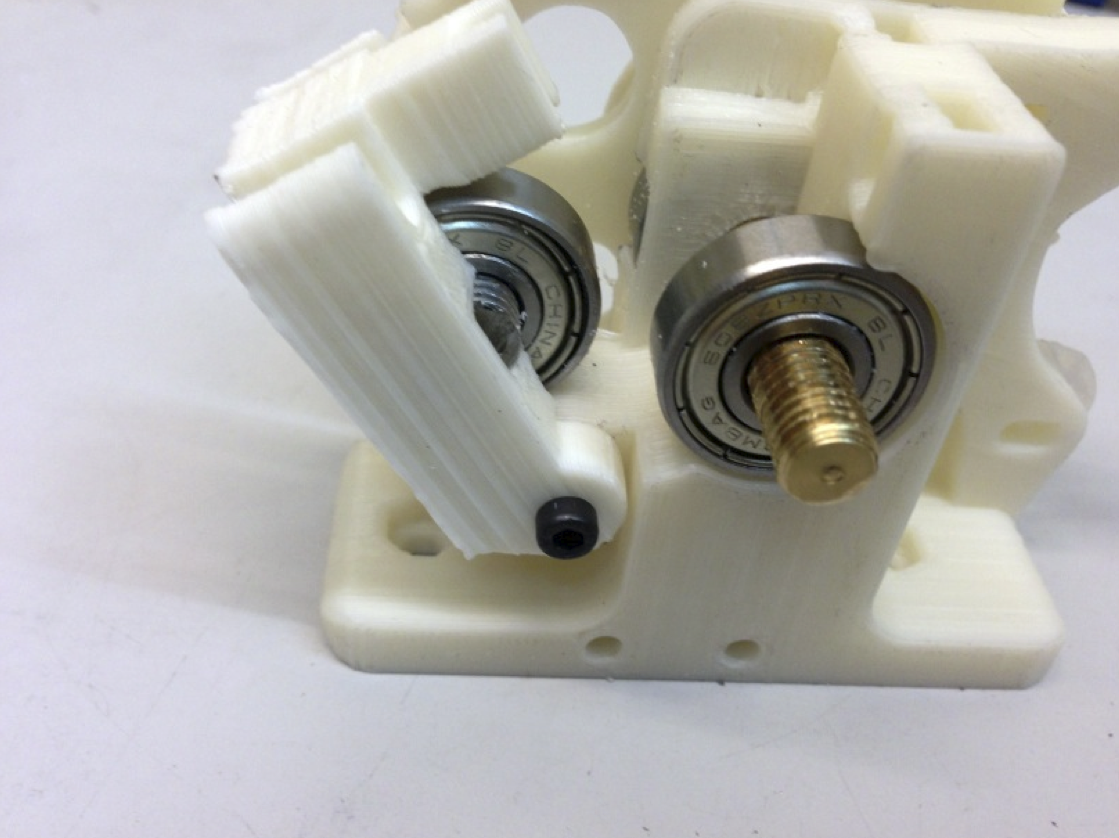
\includegraphics[width=0.7\textwidth]{../../Fotos/101.jpg}
	\caption{Detalle Idlr Extrusor }
	\label{fig:4.ext}
\end{figure}
\begin{figure}[!htp]
	\centering
	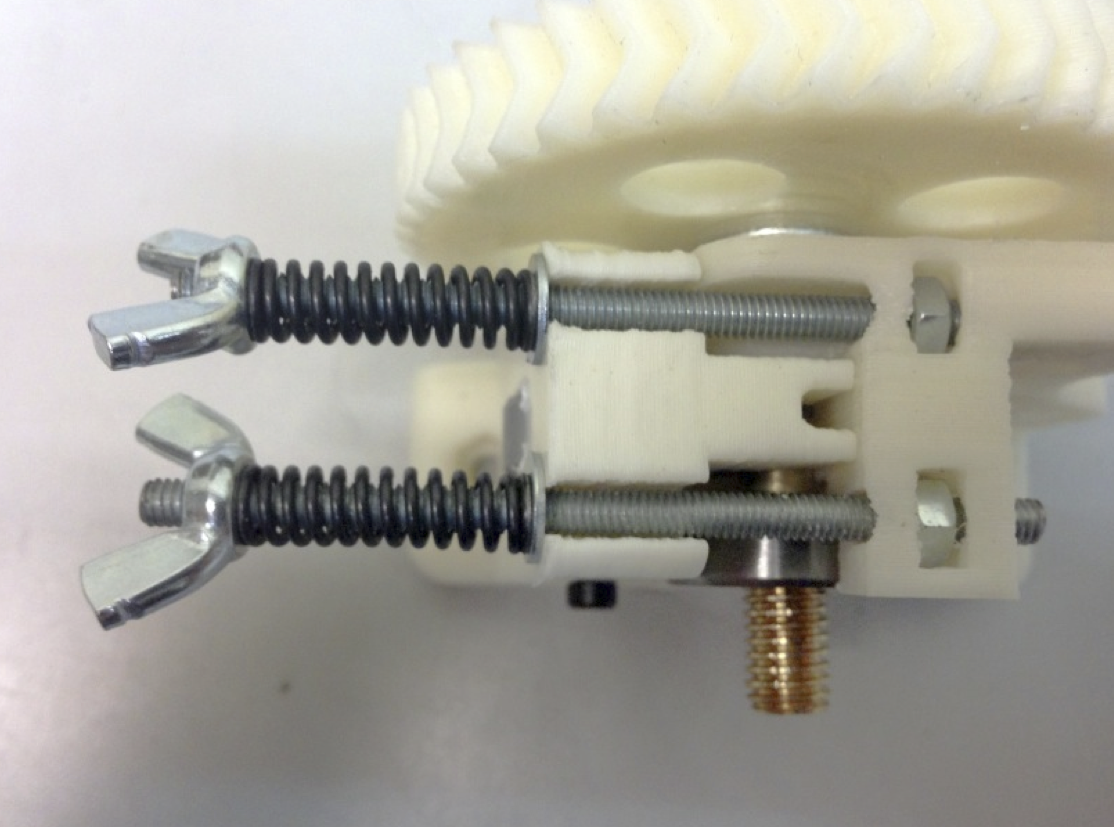
\includegraphics[width=0.7\textwidth]{../../Fotos/102.jpg}
	\caption{Extrusor finalizado}
	\label{fig:5.ext}
\end{figure}
Una vez que tenemos el cuerpo del extrusor como se muestra en la figura ~\ref{fig:5.ext} Lo atornillaremos a la pieza del eje X con dos tornillos M3x40 como se muestra en la figura ~\ref{fig:6.ext}
	\begin{figure}[!htp]
		\centering
	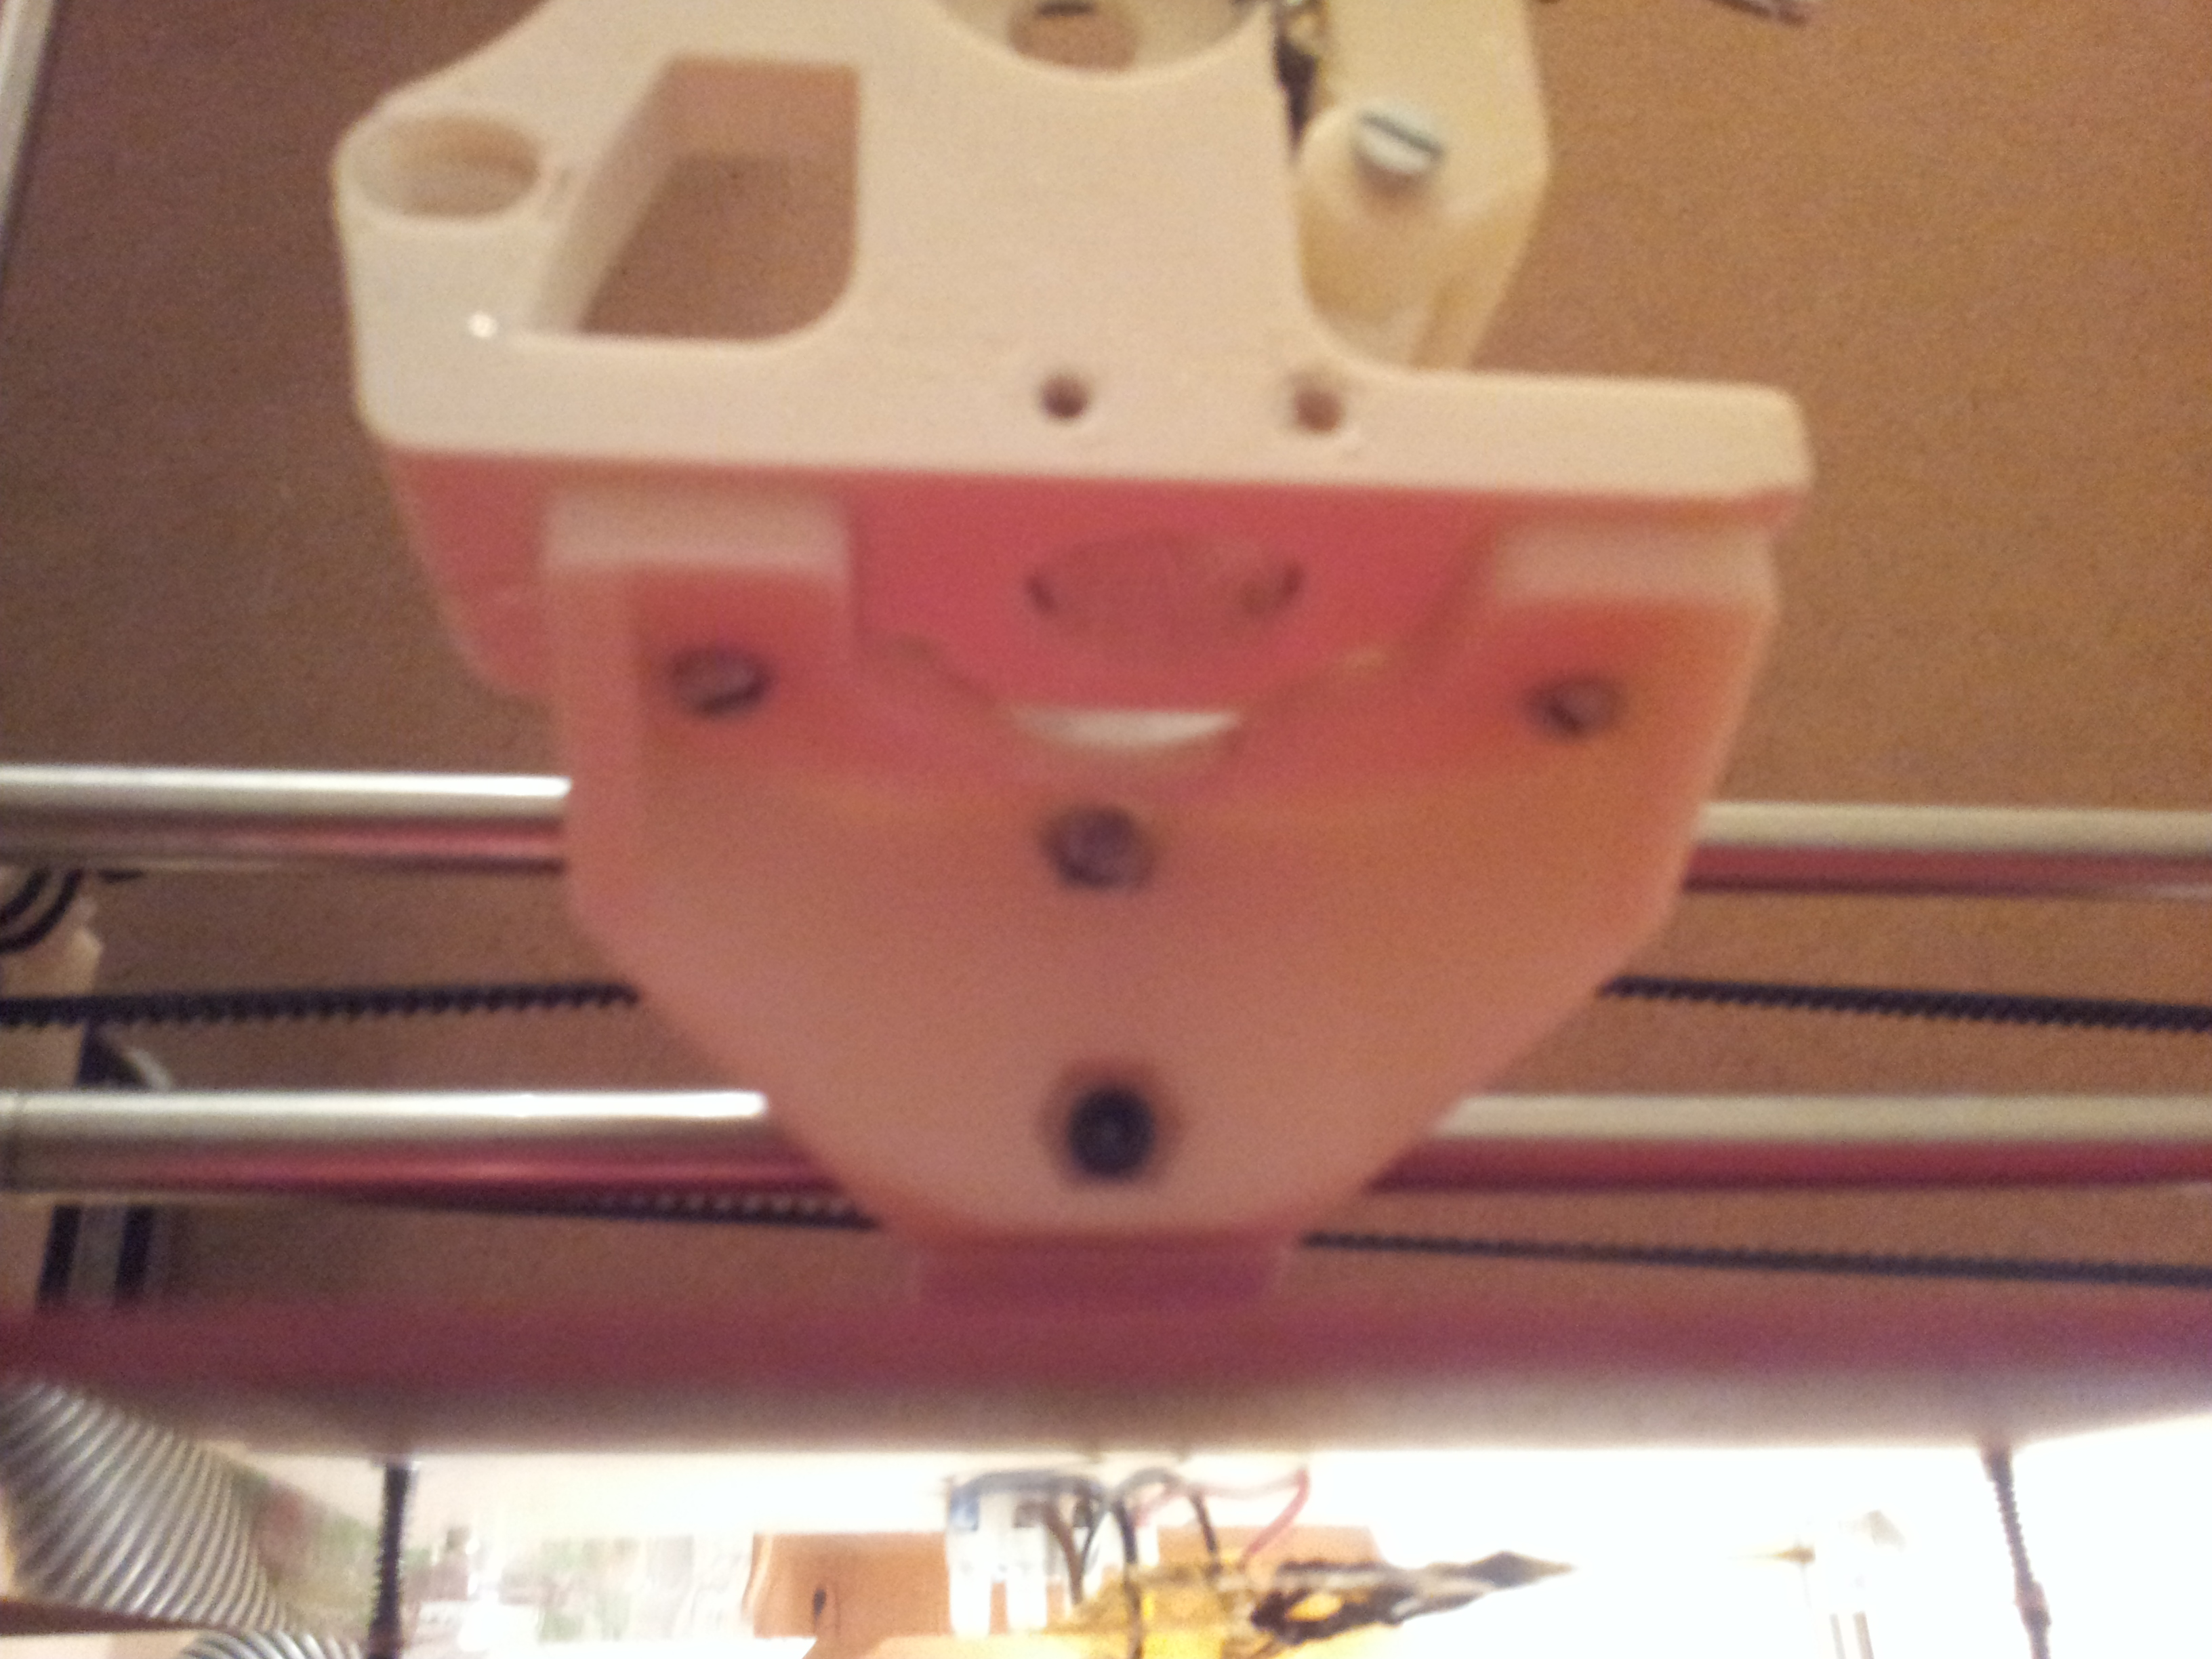
\includegraphics[width=0.7\textwidth]{../../Fotos/103.jpg}
	\caption{Cuerpo extrusor atornillado al eje X}
	\label{fig:6.ext}
\end{figure}
El siguiente paso, será atornillar el hotend al extrusor con ayuda de dos tornillos M3x40, los cables del extrusor deben quedar por la parte trasera.
\begin{figure}[!htp]
	\centering
	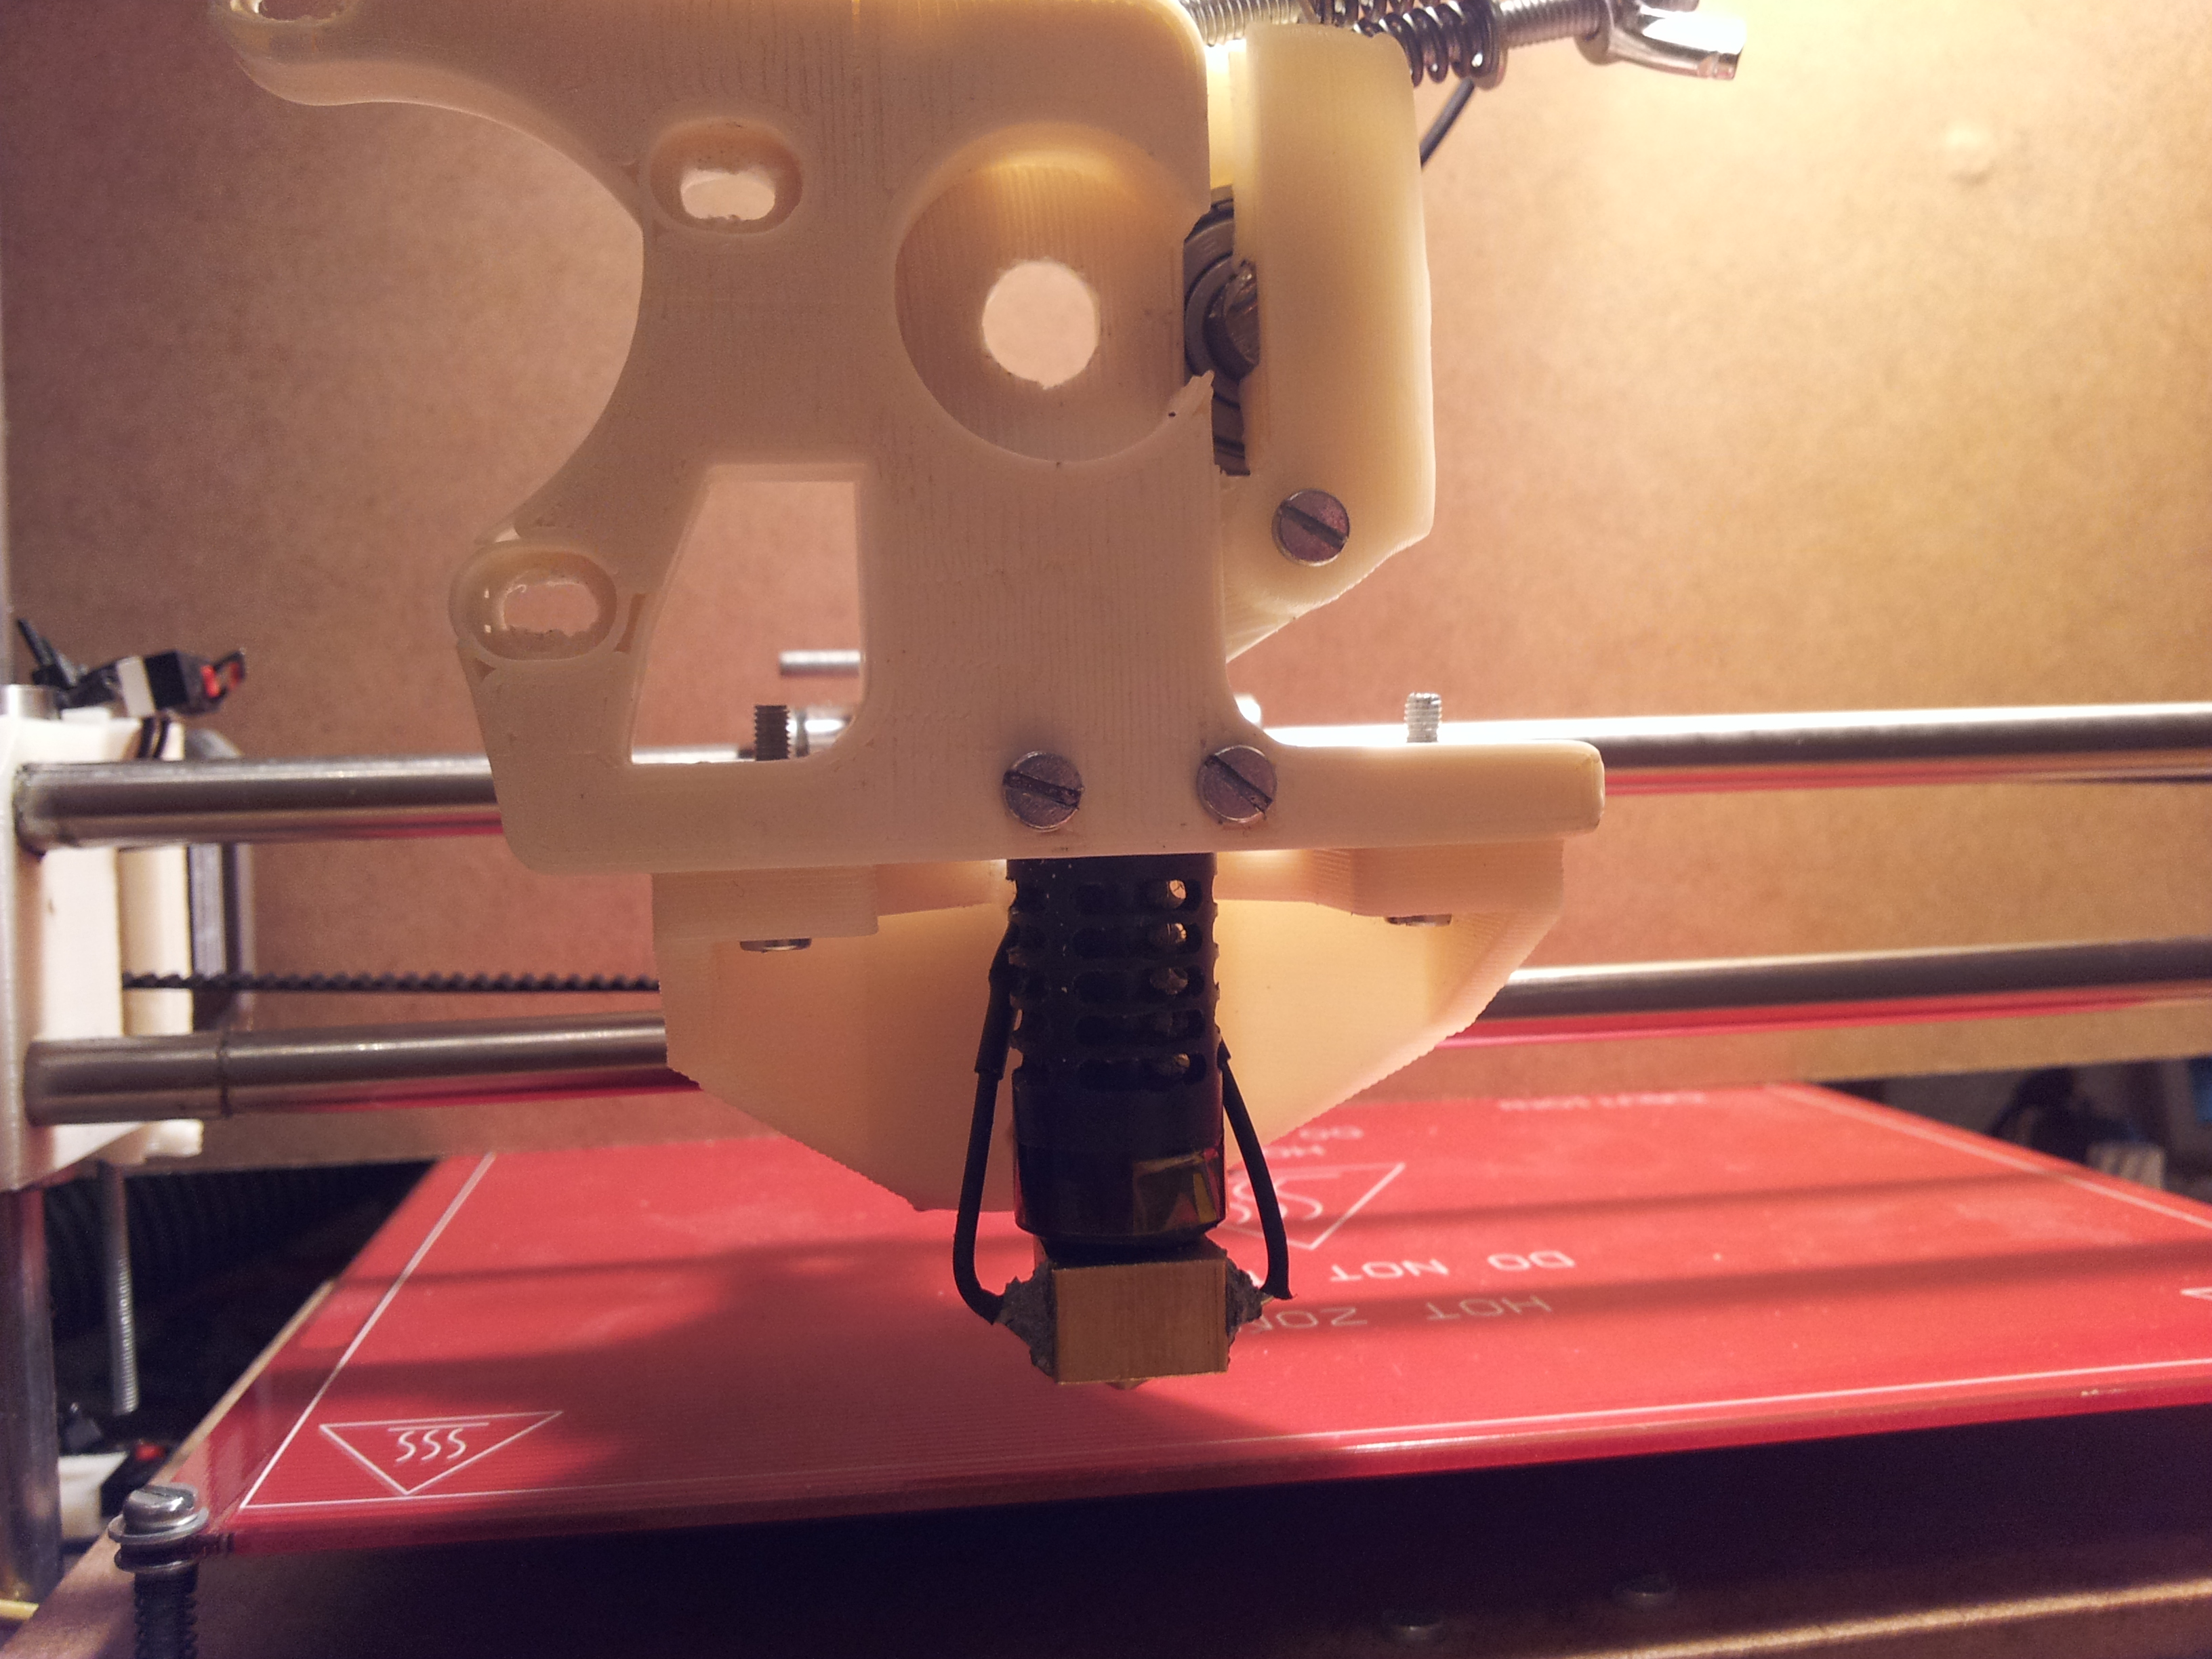
\includegraphics[width=0.7\textwidth]{../../Fotos/104.jpg}
	\caption{Hotend acoplado.}
	\label{fig:7.ext}
\end{figure}
Por último, atornillaremos el motor del extrusor con ayuda de tres tornillos M3x10. Nos deberemos asegurar en este paso, de que los dos engranajes quedan bien alineados, y a su vez, la muesca del tornillo hyena, sigue alineado con el agujero del extrusor.
\begin{figure}[!htp]
	\centering
	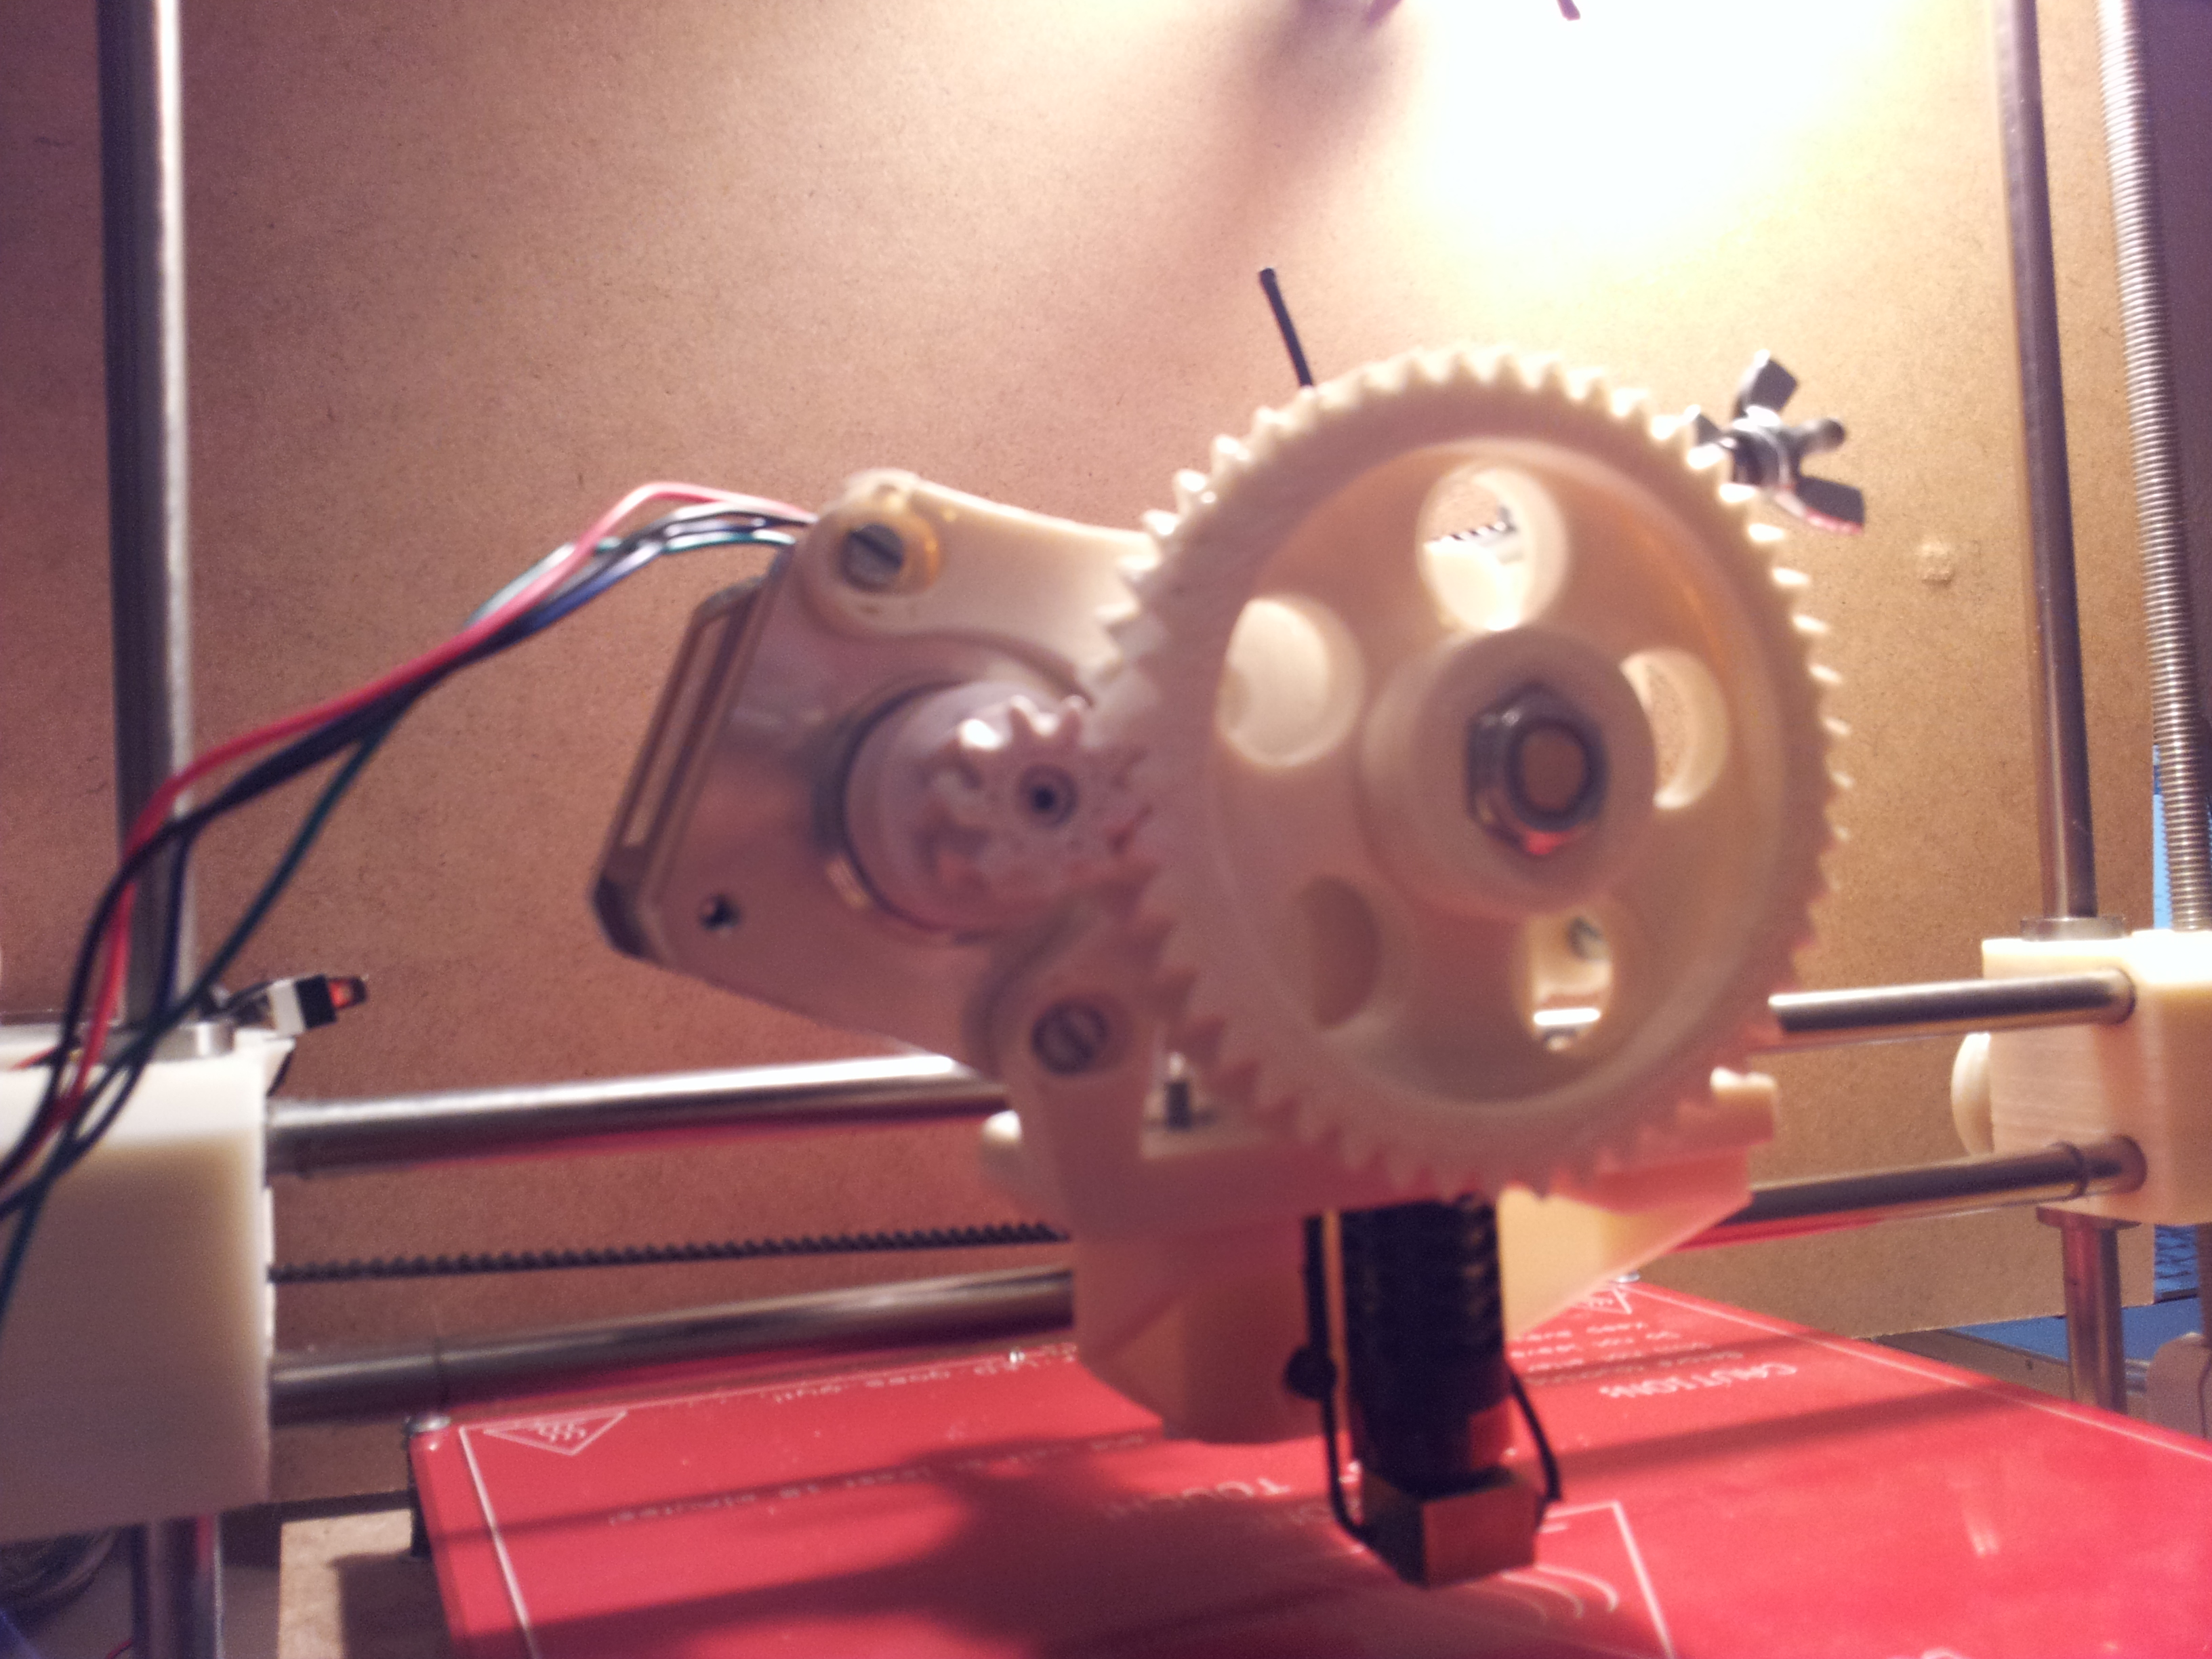
\includegraphics[width=0.7\textwidth]{../../Fotos/105.jpg}
	\caption{Extrusor finalizado}
	\label{fig:8.ext}
\end{figure}